\chapter{Chatbot}

% \section*{Customized RAG Chatbot at Aarhus University}


% In the initial phase of the project, I engaged with faculty members at Aarhus University to gain insights into the current research and application of Large Language Models (LLMs) within the university. This collaboration aimed to understand both the potential and the challenges associated with the use of LLMs in academic settings.

% Associate Professor Carsten Bergenholtz from the Department of Management contributed significantly by sharing his experiences with LLMs. His involvement provided crucial insights that shaped the direction of our project.

% \subsection*{Interview Summary}

% During our discussions, concerns were raised about the use of chatbots like ChatGPT-4 in educational environments. While these systems can produce impressive outputs, they also pose risks due to potential inaccuracies and a lack of course-specific knowledge. However, solutions exist to mitigate these challenges. Professor Bergenholtz shared his experience with implementing a customized Retrieval-Augmented Generation (RAG) chatbot for his Philosophy of Science course consisting of 550 students.

% \subsection*{Chatbot Implementation}

% The customized chatbot was used around 20,000 times by the students, indicating strong engagement and utility. Professor Bergenholtz uploaded approximately 250 pages of course-relevant documents, including text and subtitles from his lectures, to create a knowledge base for the chatbot. His setup, based on AUs Microsoft Azure platform, ensured that the chatbot was:

% \begin{itemize}
%     \item GDPR compliant, adhering to data protection regulations.
%     \item Based on the ChatGPT-4 model, ensuring advanced conversational capabilities.
%     \item Freely accessible to all students, removing financial barriers.
%     \item Equipped with an appealing user interface, enhancing user experience.
%     \item Integrated within the existing university systems, ensuring seamless access.
% \end{itemize}

% The chatbot, hosted on Aarhus University's Microsoft Azure platform, was specifically designed to respond only to queries related to the course content. Questions outside the course scope received a standard 'cannot answer this' response, maintaining the focus and academic integrity of the tool.

% \subsection*{Conclusion}

% This collaboration and the subsequent implementation of the RAG chatbot at Aarhus University exemplify the practical application of LLMs in enhancing educational experiences. The project not only addressed the immediate needs of the Philosophy of Science course but also set a precedent for future educational tools that leverage AI to support learning and inquiry.



\section*{Customized RAG Chatbot at Aarhus University}

In the initial phase of the project, I engaged with faculty members at Aarhus University to gain insights into the current research and application of Large Language Models (LLMs) within the university. This collaboration aimed to understand both the potential and the challenges associated with the use of LLMs in academic settings.

Associate Professor Carsten Bergenholtz from the Department of Management contributed significantly by sharing his experiences with LLMs. His involvement provided crucial insights that shaped the direction of our project.

\subsection*{Interview Summary}

During our discussions, concerns were raised about the use of chatbots like ChatGPT-4 in educational environments. While these systems can produce impressive outputs, they also pose risks due to potential inaccuracies and a lack of course-specific knowledge. However, solutions exist to mitigate these challenges. Professor Bergenholtz shared his experience with implementing a customized Retrieval-Augmented Generation (RAG) chatbot for his Philosophy of Science course, which had an enrollment of 550 students.

\subsection*{Chatbot Implementation}

The customized chatbot was used approximately 20,000 times by the students, indicating strong engagement and utility. Professor Bergenholtz uploaded about 250 pages of course-relevant documents, from text to subtitles from his online lectures, to create a knowledge base for the chatbot. This setup, based on AU's Microsoft Azure platform, ensured that the chatbot was:

\begin{itemize}
    \item GDPR compliant, adhering to data protection regulations.
    \item Based on the ChatGPT-4 model, ensuring advanced conversational capabilities.
    \item Freely accessible to all students, removing financial barriers.
    \item Equipped with an appealing user interface, enhancing user experience.
    \item Integrated within the existing university systems, ensuring seamless access.
\end{itemize}
\begin{figure}[H]
    \centering
    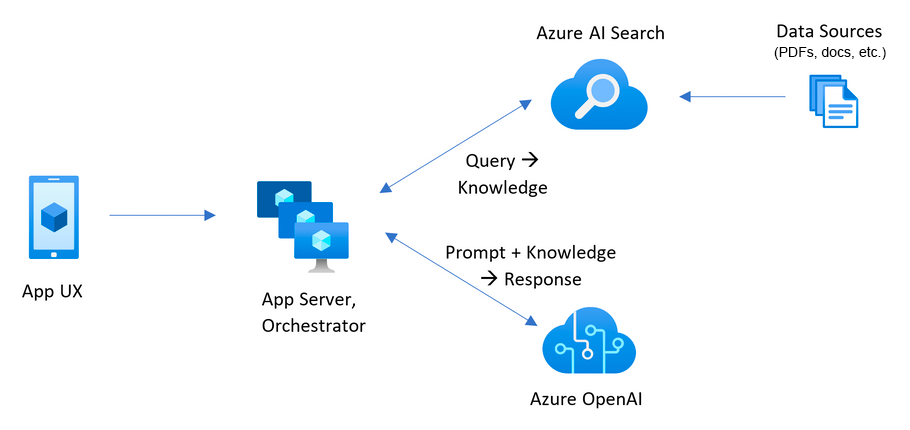
\includegraphics[width=0.6\textwidth]{figs/appcomponents.png}
    \caption{Figure to put somewhere}
    \label{fig:CLAI_Poster_Competition}
\end{figure}

The RAG chatbot was specifically designed to respond only to queries related to the course content. Questions outside the course scope received a 'cannot answer this' response to maintain the focus and academic integrity of the tool. Additionally, the chatbot provided a link to the source of its answers, enhancing transparency and trust.

\subsection*{Chatbot Evaluation and Costs}

The quality of the chatbot's responses was satisfactory, with about 85\% of interactions leading to useful answers, and only 2-4.5\% of responses being flawed. Notably, the flawed responses were quickly identified by users through follow-up questions. Despite its imperfections, the chatbot was considered a significant improvement over traditional search methods or regular chatbots used by students. The total cost of the chatbot was approximately 600€, with actual running costs around 400€ for 20,000 interactions, showcasing its cost-effectiveness.

\subsection*{Student Feedback and Future Prospects}

The chatbot was well-received based on survey responses, with students appreciating its ability to clarify complex concepts, compare texts, and summarize content. This tool proved particularly useful for large classes and when copyright for the necessary materials was held by the course instructor. Plans are in place to continue and enhance this service in future courses, focusing on guiding students to ask more effective questions.

\subsection*{Conclusion}

The implementation of the RAG chatbot at Aarhus University exemplifies the practical application of LLMs in enhancing educational experiences. The project set a precedent for future educational tools that leverage AI to support learning and inquiry. This initiative highlights the synergy between innovative technology and traditional educational practices, paving the way for more dynamic and interactive learning environments.